\section{Analisi dei requisiti}

\subsection{Definizione dei casi d'uso}
	Al momento dell'arrivo in azienda, molte componenti e funzionalità erano già parzialmente sviluppate. Alcune di esse necessitavano di adattamenti strutturali per rendere il software aderente alle norme vigenti, altre invece necessitavano di una ristrutturazione dell'interfaccia utente. \\ 
	Per la maggior parte del tempo si è sviluppato lato back-end  ma, dal momento che l'obiettivo dello stage è stato consolidare il sistema per permettere il rilascio di una versione alpha, sono stati trattati anche aspetti lato front-end. 
	Sono stati dunque riportati nei casi d'uso tutti gli aspetti toccati durante lo stage,  specificando nella descrizione le modifiche che sono state apportate alla componente interessata. \\ 
	I casi  d'uso per i quali è stata eseguita un riprogettazione sono stati differenziati da quelli per i quali era necessaria una soluzione da zero mediante il colore di sfondo.
	\subsubsection{Legenda}
	Sono stati rappresentati con sfondo azzurro i casi d'uso per i quali è stato eseguita una riprogettazione; quelli su sfondo bianco  invece hanno richiesto progettazione e sviluppo di una soluzione da zero.
	\begin{itemize}
		\item \textit{Notazione di caso d'uso relativo a  componenti progettate da zero:}
		\begin{figure}[H]
			\begin{center}
				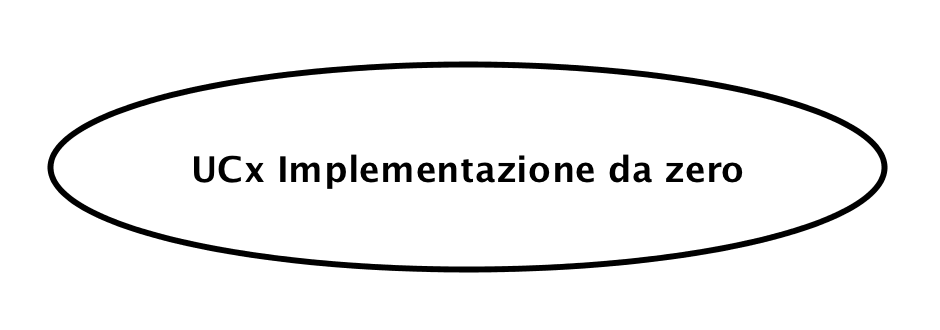
\includegraphics[width=7cm]{Pics/UCDaZero.png}
				\caption{Notazione di caso d'uso  relativo ad una componenti progettate da zero;}
				\label{fig:DiagrammaUCDaZero}
			\end{center}
		\end{figure}
		\item \textit{Caso d'uso relativo a componenti riprogettate dal punto di vista strutturale o dell'interfaccia utente:}
				 	\begin{figure}[H]
				 		\begin{center}
				 			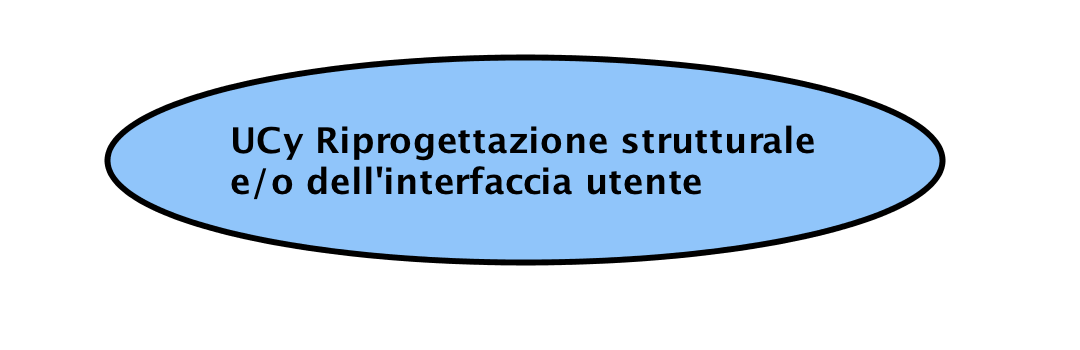
\includegraphics[width=8cm]{Pics/UCRestaurato.png}
				 			\caption{Notazione di caso d'uso relativo a componenti riprogettate.}
				 			\label{fig:DiagrammaUCRiprogettato}
				 		\end{center}
				 	\end{figure}		
	\end{itemize}
	\newpage
	\subsubsection{Attori}
	\begin{figure}[H]
		\begin{center}
			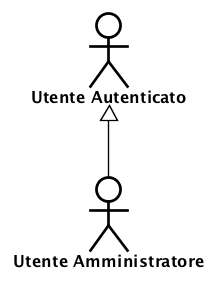
\includegraphics[width=5cm]{Pics/Attori.png}
			\caption{Attori coinvolti.}
			\label{fig:DiagrammaAttori}
		\end{center}
	\end{figure}	
	Sono state individuate due categorie di attori: 
	\begin{itemize}
		\item \texttt{Utente amministratore:} Utente che ha effettuato con successo il login nel sistema con privilegi da amministratore;
		\item \texttt{Utente autenticato:} Utente che ha effettuato con successo il login nel sistema.
	\end{itemize}
	
	L'\texttt{utente amministratore} specializza l'\texttt{utente autenticato}.
	
	\newpage
	\subsubsection{Caso d'uso UCP - Scenario Principale }
	\begin{figure}[H]
		\begin{center}
			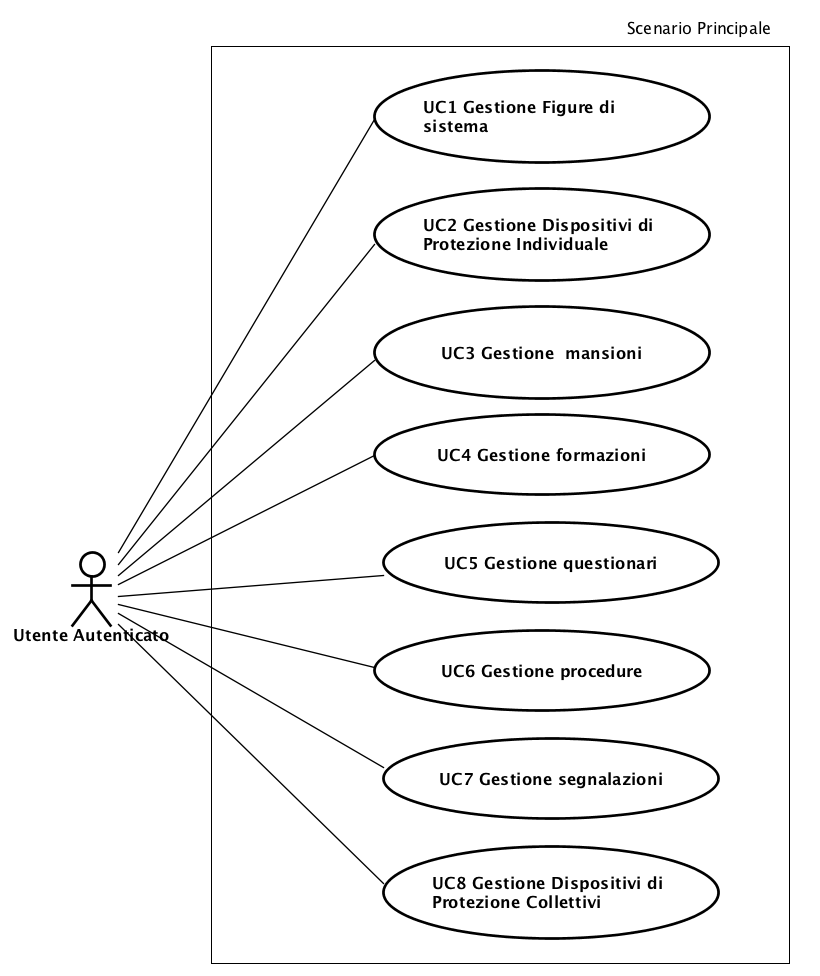
\includegraphics[width=11cm]{Pics/Diagramma_generale_dei_casi_d_uso.png}
			\caption{
				Diagramma dei casi d'uso generale.}
			\label{fig:DiagrammaGeneraleCasiDuso}
		\end{center}
	\end{figure}	
	
	\begin{itemize}
		\item \textbf{Scopo:} Il diagramma generale dei casi d'uso UCP (\autoref{fig:DiagrammaGeneraleCasiDuso}), ha lo scopo di rappresentare ad alto livello i casi d'uso necessari al soddisfacimento di tutti i requisiti. \\
		In particolare un utente che abbia effettuato con successo il login nel sistema, deve poter gestire: figure di sistema; dispositivi di protezione individuali, mansioni, formazioni, questionari, procedure; segnalazioni e dispositivi di protezione collettivi.
		A seguire la spiegazione e l'esplosione in sotto casi d'uso per ognuno dei casi d'uso sopra elencati.
		\item \textbf{Attori Coinvolti:} Utente Autenticato;
		\item \textbf{Flusso principale degli eventi:} 
			\begin{itemize}
				\item \textit{L'utente autenticato gestisce le Figure di sistema (\hyperref[section:UC1]{UC1});}
				\item \textit{L'utente autenticato gestisce i Dispositivi di Protezione Individuale (\hyperref[section:UC2]{UC2});}
				\item \textit{L'utente autenticato gestisce le mansioni (\hyperref[section:UC3]{UC3});}
				\item \textit{L'utente autenticato gestisce le formazioni (\hyperref[section:UC4]{UC4});}
				\item \textit{L'utente autenticato gestisce le procedure (\hyperref[section:UC5]{UC5});}
				\item \textit{L'utente autenticato gestisce le segnalazioni (\hyperref[section:UC6]{UC6})}
				\item \textit{L'utente autenticato gestisce i Dispositivi di Protezione Collettivi (\hyperref[section:UC7]{UC7}).}
			\end{itemize}
	\end{itemize}
	

	\subsubsection{UC1 Gestione delle Figure di sistema}
	\label{section:UC1}
	\begin{figure}[H]
		\begin{center}
			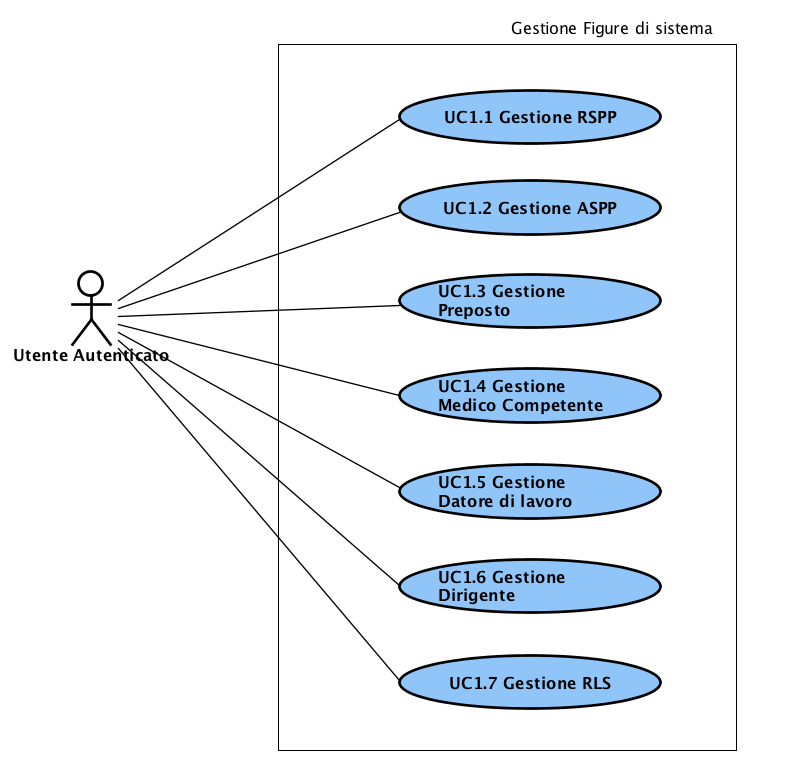
\includegraphics[width=12cm]{Pics/UC1GestioneFigureDiSistema.png}
			\caption{
				Diagramma dei casi d'uso UC1 - Figure di sistema.}
			\label{fig:UC1GestioneFigureDiSistema}
		\end{center}
	\end{figure}
	\begin{itemize}
		\item \textbf{Scopo:} Il diagramma generale dei casi d'uso UC1 (\autoref{fig:UC1GestioneFigureDiSistema}), ha lo scopo di rappresentare ad alto livello i casi d'uso necessari al soddisfacimento di tutti i requisiti rigruardanti le figure di sistema;
		\item \textbf{Attori Coinvolti:} Utente Autenticato;
		\item \textbf{Flusso principale degli eventi:} 
		\begin{itemize}
			\item \textit{L'utente autenticato gestisce gli \gls{RSPP}\G\ (\hyperref[section:UC1_1]{UC1.1});}
			\item \textit{L'utente autenticato gestisce gli \gls{ASPP}\G\ (UC1.2);}
			\item \textit{L'utente autenticato gestisce i preposti (UC1.3);}
			\item \textit{L'utente autenticato gestisce il medico competente (UC1.4);}
			\item \textit{L'utente autenticato gestisce il datore di lavoro (UC1.5);}
			\item \textit{L'utente autenticato gestisce i dirigenti (UC1.6);}
			\item \textit{L'utente autenticato gestisce gli \gls{RLS}\G\  (UC1.7).}
		\end{itemize}
	\end{itemize}
	
	\newpage
	\subsubsection{UC1.1 Gestione degli RSPP}
	\label{section:UC1_1}
	Tutte le figure di sistema presentano requisiti analoghi. Per evitare di affaticare la lettura con sezioni ridondanti è stato scelto di riportare soltanto il diagramma dei casi d'uso riguardante gli \gls{RSPP}\G. Si intende che per tutte le altre figure di sistema il diagramma sia analogo. 
		\begin{figure}[H]
			\begin{center}
				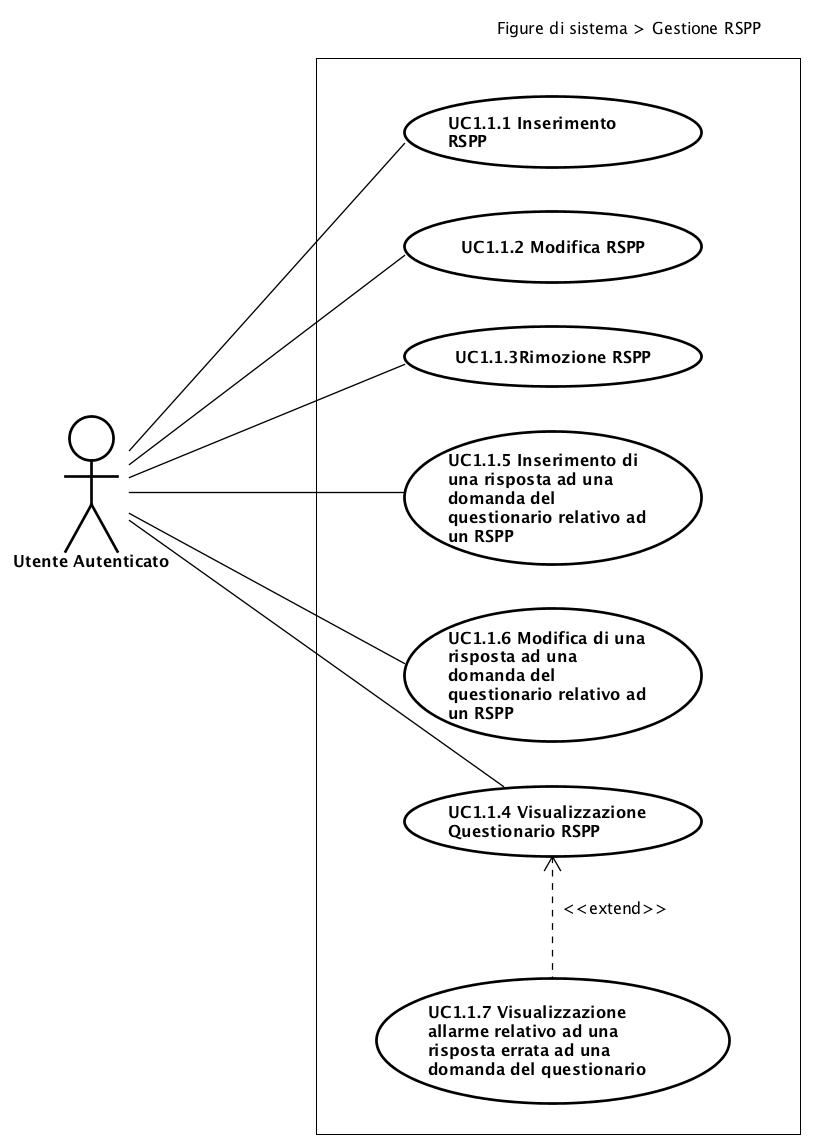
\includegraphics[width=12cm]{Pics/UC1_1_FigureDiSistema_RSPP.png}
				\caption{Diagramma dei casi d'uso relativo all'inserimento degli RSPP}
				\label{fig:UC1_1RSPP}
			\end{center}
		\end{figure}
		\begin{itemize}
			\item \textbf{Scopo:} Il diagramma relativo alla gestione degli RSPP (\autoref{fig:DiagrammaGeneraleCasiDuso}), ha lo scopo di rappresentare i casi d'uso necessari al soddisfacimento di tutti i requisiti riguardanti la gestione degli RSPP. \\
			In particolare un utente che abbia effettuato con successo il login nel sistema, deve poter inserire, rimuovere, modificare  \gls{RSPP}\G. Deve essere messo in condizione inoltre di Visualizzare un questionario relativo ad uno specifico \gls{RSPP}\G, rispondendo alle domande riportate su di esso. In caso di errore, deve essere sollevato un allarme che comunica la domanda esatta ed un messaggio esplicativo.
			\item \textbf{Attori Coinvolti:} Utente Autenticato;
			\item \textbf{Flusso principale degli eventi:} 
			\begin{itemize}
				\item \textit{L'utente autenticato inserisce un \gls{RSPP}\G\ (UC1.1.1);}
				\item \textit{L'utente autenticato modifica un \gls{RSPP}\G\ (UC1.1.2);}
				\item \textit{L'utente autenticato rimuove un \gls{RSPP}\G\  (UC1.1.3);}
				\item \textit{L'utente autenticato visualizza il questionario associato ad un \gls{RSPP}\G\  (UC1.1.4);}
				\item \textit{L'utente autenticato inserisce una risposta ad una domanda del questionario (UC1.1.5);}
				\item \textit{L'utente autenticato modifica di una risposta ad una domanda del questionario relativo ad un \gls{RSPP}\G\  (UC1.1.6);}
				\item \textit{ L'utente autenticato visualizza un allarme relativo ad una risposta errata ad una domanda del questionario (UC1.1.7).}
			\end{itemize}
		\end{itemize}
	\newpage	
	\subsubsection{UC2 Gestione dei DPI}
		\label{section:UC2}
		La gestione dei  \gls{DPI}\G\ va suddivisa in due scenari distinti. Il primo scenario è relativo alla gestione delle tipologie di \gls{DPI}\G\ disponibili da parte degli utenti amministratori. Il secondo scenario riguarda la gestione dei \gls{DPI}\G\ che compongono la dotazione personale di un dipendente. \\
		Seguono i diagrammi dei casi d'uso dei \gls{DPI}\G\ relativi agli scenari sopra indicati.

		\paragraph*{UC2.1 Gestione delle tipologie di DPI dal pannello di amministrazione }\mbox{} \\
			\label{section:UC2_1}
			\begin{figure}[H]
				\begin{center}
					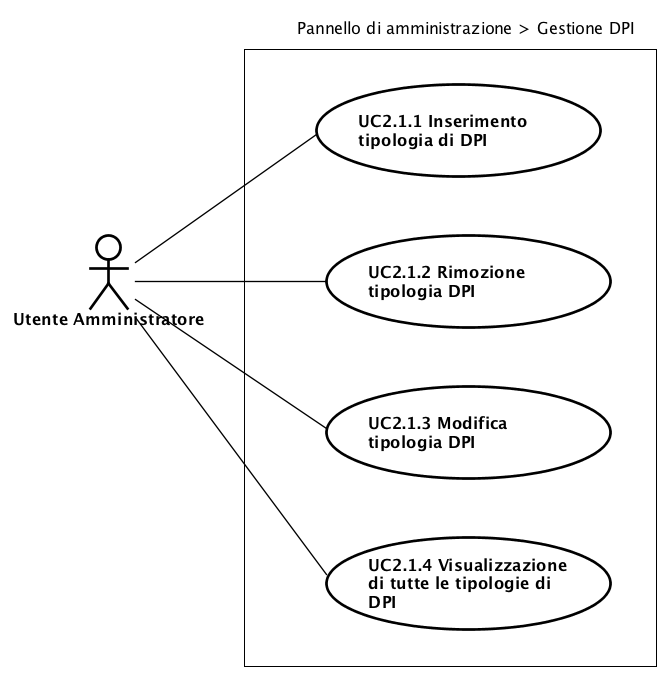
\includegraphics[width=12cm]{Pics/UC2_1GestioneDispositiviDiProtezioneIndividualeDaPannelloDiAmministrazione.png}
					\caption{
						Diagramma dei casi d'uso UC2.1 - Gestione tipologie di DPI dal pannello di amministrazione.}
					\label{fig:UC2_1GestioneDPIAmministrazione}
				\end{center}
			\end{figure}
			\begin{itemize}
				\item \textbf{Scopo:} Il diagramma presentato nella \autoref{fig:UC2_1GestioneDPIAmministrazione}, ha lo scopo di rappresentare i casi d'uso necessari al soddisfacimento di tutti i requisiti riguardanti la gestione delle tipologie dei \gls{DPI}\G.
				 \\ Un utente amministratore deve poter gestire in modo autonomo le tipologie di \gls{DPI}\G\ che ritiene più opportune e metterle a disposizione degli utilizzatori del sistema.
				\item \textbf{Attori Coinvolti:} Utente Amministratore;
				\item \textbf{Flusso principale degli eventi:} 
				\begin{itemize}
					\item \textit{L'utente amministratore inserisce una tipologia di \gls{DPI}\G\ (UC2.1.1);}
					\item \textit{L'utente amministratore rimuove una tipologia di \gls{DPI}\G\ (UC2.1.2);}
					\item \textit{L'utente amministratore modifica una tipologia di \gls{DPI}\G\ (UC2.1.3);}
					\item \textit{L'utente amministratore visualizza tutte le tipologie di \gls{DPI}\G\ (UC2.1.3).}
				\end{itemize}
			\end{itemize}
		\paragraph*{UC2.2 Gestione dei DPI assegnati ai dipendenti}\mbox{} \\
			\label{section:UC2_2}
			\begin{figure}[H]
				\begin{center}
					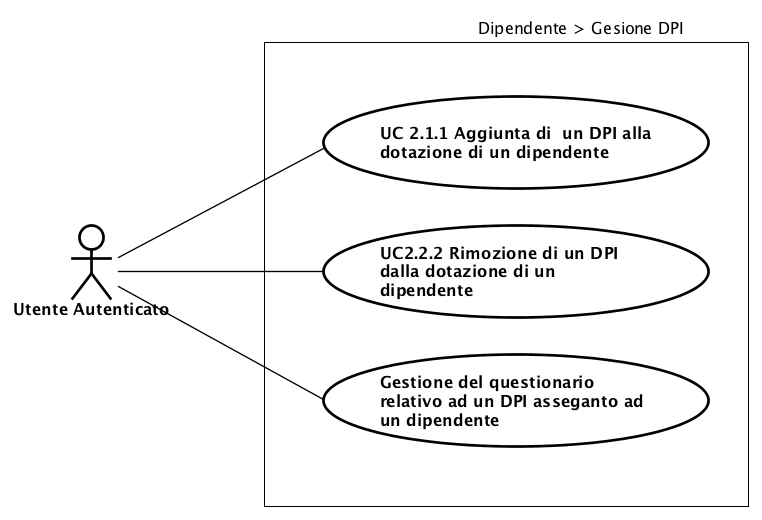
\includegraphics[width=12cm]{Pics/UC2_2DPIDipendenti.png}
					\caption{
						Diagramma dei casi d'uso UC2.2 - Gestione dei DPI relativi ad un dipendente.}
					\label{fig:UC2_2GestioneDPIDipendenti}
				\end{center}
			\end{figure}
			\begin{itemize}
				\item \textbf{Scopo:} Il diagramma presentato nella \autoref{fig:UC2_2GestioneDPIDipendenti}, ha lo scopo di rappresentare i casi d'uso necessari al soddisfacimento di tutti i requisiti riguardanti la gestione dei \gls{DPI}\G\ dati in dotazione ai dipendenti. \\ Un utente autenticato deve poter assegnare o rimuovere \gls{DPI}\G\ ad ogni dipendente. Deve essere possibile assegnare \gls{DPI}\G\ con molteplicità variabile, scegliendo la tipologia da una lista predefinita (Sezione: \ref{section:UC2_1}).\\
				Per ogni \gls{DPI}\G\ deve essere possibile rispondere ad un questionario;
				\item \textbf{Attori Coinvolti:} Utente Autenticato;
				\item \textbf{Flusso principale degli eventi:} 
				\begin{itemize}
					\item \textit{L'utente autenticato aggiunge un \gls{DPI}\G\ alla dotazione di un dipendente (UC2.2.1);}
					\item \textit{L'utente autenticato rimuove un \gls{DPI}\G\ dalla dotazione di un dipendente  (UC2.2.2);}
					\item \textit{L'utente autenticato gestisce il questionario relativo ad un \gls{DPI}\G\ assegnato ad un dipendente (UC2.2.3);}
					\item \textit{L'utente autenticato visualizza tutti i \gls{DPI}\G\ assegnati ad un dipendente (UC2.2.4).}
				\end{itemize}
			\end{itemize}
	
	\newpage		
	\subsubsection{UC3 Gestione  delle mansioni}
		\label{section:UC3}
		Le mansioni rappresentano le attività che un individuo interno all'azienda è abilitato a svolgere.\\
		L'associazione agli individui e la gestione delle mansioni disponibili è stato eseguito allo stesso modo dei \gls{DPI}\G. \\
		Per evitare di affaticare la lettura con sezioni ridondanti è stato scelto di riportare soltanto il diagramma dei casi d'uso riguardante i \gls{DPI}\G. Si intende che per le mansioni il diagramma e la spiegazione del caso d'uso sia analogo alla sezione \ref{section:UC2_2}.\\
		\newpage 
	\subsubsection{UC4 Gestione delle formazioni}
		\label{section:UC4}
		Con il termine formazione si intende una certificazione relativa ad un corso abilitante ad una o più mansioni.\\
		La gestione delle formazioni è del tutto simile a quella dei \gls{DPI}\G, fatta eccezione per la gestione delle scadenze. È richiesto infatti che un utente amministratore possa assegnare un periodo di validità della formazione in mesi dal pannello di controllo. Un utente autenticato deve visualizzare un allarme nel momento in cui una formazione sia scaduta.

	\paragraph*{UC4.1 Gestione delle formazioni dal pannello di amministrazione }\mbox{} \\
		\label{section:UC4_1}
		Tutte le considerazioni della sezione \ref{section:UC2} valgono anche per le formazioni. \\
		A differenza dei \gls{DPI}\G\ va inserita una informazione aggiuntiva obbligatoria: il periodo di validità della formazione. \\
		Il diagramma dei casi d'uso è del tutto analogo a quello della  \autoref{fig:UC2_1GestioneDPIAmministrazione}.
	\paragraph*{UC4.2 Gestione delle formazioni dei dipendenti e del datore di lavoro }\mbox{} \\
		\label{section:UC4_2}
		\begin{figure}[H]
			\begin{center}
				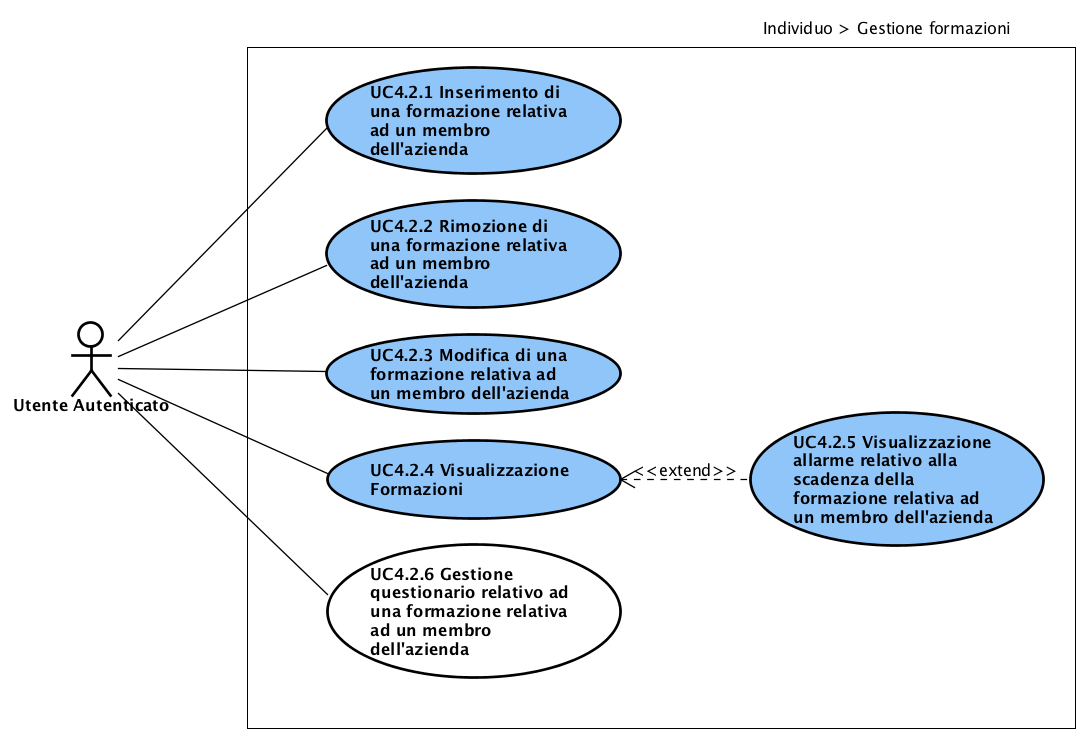
\includegraphics[width=16cm]{Pics/UC4_2GestioneFormazioni.png}
				\caption{Diagramma dei casi d'uso relativo alla gestione delle formazioni di un dipendente.}
				\label{fig:UC4_2_Formazioni}
			\end{center}
		\end{figure}
		
		\begin{itemize}
			\item \textbf{Scopo:} Il diagramma presentato nella \autoref{fig:UC4_2_Formazioni}, ha lo scopo di rappresentare i casi d'uso necessari al soddisfacimento di tutti i requisiti riguardanti la gestione delle formazioni relative ad un qualunque membro dell'azienda. \\ 
			Un utente autenticato deve poter assegnare o rimuovere formazioni ad ogni dipendente. 
			Ogni formazione relativa ad un dipendente deve essere dotata di un questionario. \\ 
			La scadenza della formazione deve essere segnalata trenta giorni prima della data ultima mediante un allarme.
			\item \textbf{Attori Coinvolti:} Utente Autenticato;
			\item \textbf{Flusso principale degli eventi:} 
			\begin{itemize}
				\item \textit{L'utente autenticato aggiunge una formazione ad un membro dell'azienda indicando descrizione e data (UC4.2.1);}
				\item \textit{L'utente autenticato rimuove una formazione ad un membro dell'azienda (UC4.2.2);}
				\item \textit{L'utente autenticato modifica una formazione ad un membro dell'azienda (UC4.2.3);}
				\item \textit{L'utente autenticato visualizza le formazioni relative ad un membro dell'azienda (UC4.2.4);}
				\item \textit{L'utente autenticato visualizza l'allarme relativo alla scadenza di una formazione in possesso di un membro dell'azienda (UC4.2.5);}
				\item \textit{L'utente autenticato gestisce il questionario relativo ad una formazione in possesso di un membro dell'azienda (UC4.2.6).}
			\end{itemize}
		\end{itemize}
	\newpage	
%	\subsubsection{UC5 Gestione dei questionari}
%	\hl{TODO Rimuovere e sistemare tutta la numerazione degli uc successivi + riferimenti nella tabella dei requisiti}
%	
%		\label{section:UC5}	
%			\begin{figure}[H]
%				\begin{center}
%					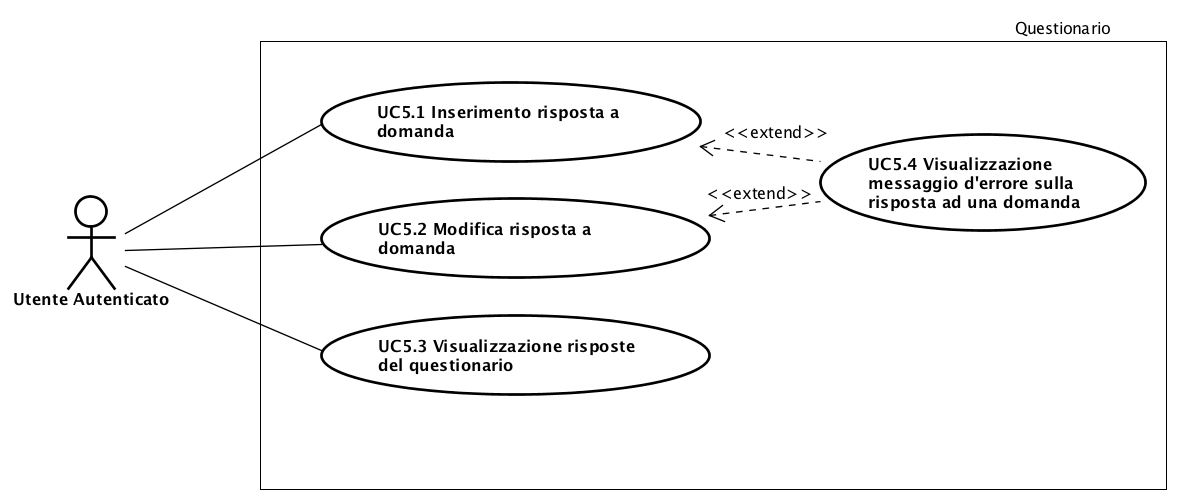
\includegraphics[width=15cm]{Pics/UC5QuestionarioUtenteAutenticato.png}
%					\caption{Diagramma dei casi d'uso relativo alla gestione di un questionario.}
%					\label{fig:UC5_Qestionari}
%				\end{center}
%			\end{figure}
%			
%			\begin{itemize}
%				\item \textbf{Scopo:} Il diagramma presentato nella \autoref{fig:UC5_Qestionari}, ha lo scopo di rappresentare i casi d'uso necessari al soddisfacimento dei requisiti riguardanti la gestione di un questionario di pertinenza di un utente autenticato. \\ 
%				Gli utenti amministratori devono poter gestire le domande poste nei questionari da un pannello d'amministrazione. Questo aspetto non è stato trattato in dettaglio poiché analogo a quanto descritto nella sezione \ref{section:UC2_1}.
%				\item \textbf{Attori Coinvolti:} Utente Autenticato;
%				\item \textbf{Flusso principale degli eventi:} 
%				\begin{itemize}
%					\item \textit{L'utente autenticato risponde per la prima volta ad una domanda (UC5.1);}
%					\begin{itemize}
%						\item \textit{Viene mostrato un messaggio d'errore se la risposta fornita non è corretta (UC5.4);}
%					\end{itemize}
%					\item \textit{L'utente autenticato modifica una risposta ad una domanda (UC5.2);}
%					\begin{itemize}
%						\item \textit{Viene mostrato un messaggio d'errore se la risposta fornita non è corretta (UC5.4);}
%					\end{itemize}
%					\item \textit{L'utente autenticato visualizza tutte le risposte al questionario (UC5.3). Se è la prima volta che lo apre, le risposte saranno tutte vuote.}
%				\end{itemize}
%			\end{itemize}
%


	\newpage		
	\subsubsection{UC5 Gestione delle procedure}
		\label{section:UC5}
		Le procedure rappresentano un aspetto di primaria importanza e si suddividono in due categorie: di prassi e di sistema. \\
		Le procedure di prassi derivano direttamente da un documento fornito dall'\gls{INAIL}\G. Queste procedure sono state individuate dall'analisi delle cause di infortunio maggiormente frequenti rilevate dall'\gls{INAIL}\G\ nel tempo allo scopo di migliorare la sicurezza dei lavoratori.
		Le procedure di sistema, invece, sono stese dall'azienda e fanno parte del \gls{DVR}\G. 
		\begin{figure}[H]
			\begin{center}
				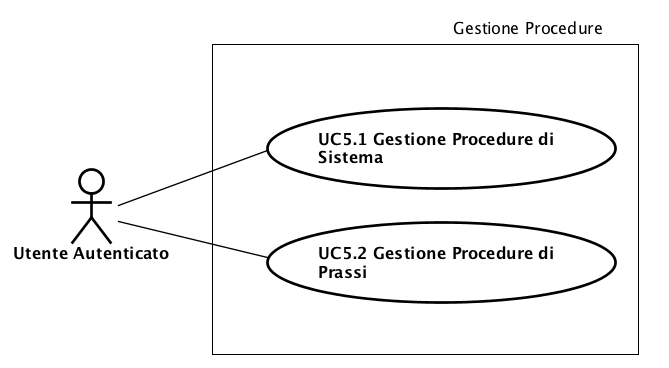
\includegraphics[width=12cm]{Pics/UC5GestioneProcedure.png}
				\caption{Diagramma dei casi d'uso relativo alla gestione delle procedure.}
				\label{fig:UC5_Procedure}
			\end{center}
		\end{figure}
		
			\begin{itemize}
				\item \textbf{Scopo:} Il diagramma presentato nella \autoref{fig:UC5_Procedure}, ha lo scopo di rappresentare i casi d'uso necessari alla gestione delle procedure all'interno dell'azienda. \\ 
				
				Un utente autenticato deve poter gestire le procedure di ogni dipendente dell'azienda. \\
				Ogni procedura, di sistema, deve essere dotata di descrizione, codifica ed informazioni relative alle revisioni delle quali è stata oggetto nel tempo.\\
				Le procedure di prassi sono state gestite con un questionario in quanto derivanti direttamente da una lista di domande proveniente dall'\gls{INAIL}\G;
				\item \textbf{Attori Coinvolti:} Utente Autenticato;
				\item \textbf{Flusso principale degli eventi:} 
				\begin{itemize}
					\item \textit{L'utente autenticato gestisce le procedure di sistema(UC5.1);}
					\begin{itemize}
						\item \textit{L'utente autenticato inserisce una nuova procedura di sistema(UC5.1.1);}
						\item \textit{L'utente autenticato modifica una procedura di sistema(UC5.1.2);}
						\item \textit{L'utente autenticato rimuove una procedura di sistema(UC5.1.3);}
						\item \textit{L'utente autenticato visualizza tutte le procedure di sistema(UC5.1.4).}
					\end{itemize}
					\item \textit{L'utente autenticato gestisce le procedure di prassi (UC5.2);}
					\begin{itemize}
						\item \textit{L'utente autenticato inserisce una nuova procedura di prassi (UC5.2.1);}
						\item \textit{L'utente autenticato modifica una procedura di prassi (UC5.2.2);}
						\item \textit{L'utente autenticato rimuove una procedura di prassi (UC5.2.3);}
						\item \textit{L'utente autenticato visualizza tutte le procedure di prassi (UC5.2.4).}
					\end{itemize}
				\end{itemize}
			\end{itemize}
			
	\newpage
	\subsubsection{UC6 Gestione delle segnalazioni}
		\label{section:UC6}	
		Le segnalazioni sono delle comunicazioni ufficiali indirizzate all'organo di vigilanza. Esse sono dotate di: descrizione, segnalante, data di comunicazione del segnalante all'alta direzione, data di comunicazione dall'alta direzione all'organo di vigilanza, data di risposta dell'organo di vigilanza al soggetto interessato.\\
		\begin{figure}[H]
			\begin{center}
				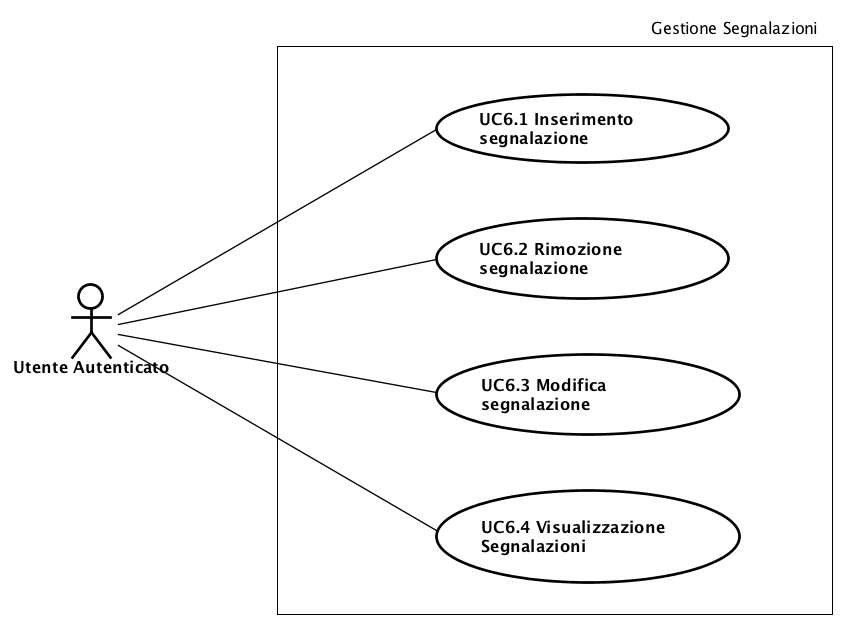
\includegraphics[width=12cm]{Pics/UC6Segnalazioni.png}
				\caption{Diagramma dei casi d'uso relativo alla gestione delle segnalazioni.}
				\label{fig:UC6_Segnalazioni}
			\end{center}
		\end{figure}
		
		\begin{itemize}
			\item \textbf{Scopo:} Il diagramma presentato nella \autoref{fig:UC6_Segnalazioni}, ha lo scopo di rappresentare i casi d'uso necessari al soddisfacimento di tutti i requisiti riguardanti la gestione delle segnalazioni all'interno dell'azienda. \\ 
			\item \textbf{Attori Coinvolti:} Utente Autenticato;
			\item \textbf{Flusso principale degli eventi:} 
			\begin{itemize}
				\item \textit{L'utente autenticato inserisce una segnalazione (UC6.1);}
				\item \textit{L'utente autenticato rimuove una segnalazione (UC6.2);}
				\item \textit{L'utente autenticato modifica una segnalazione (UC6.3);}
				\item \textit{L'utente autenticato visualizza tutte le segnalazioni (UC6.4);}
			\end{itemize}
		\end{itemize}
		
	\newpage	
	\subsubsection{UC7 Gestione dei Dispositivi di Protezione Collettivi}
		\label{section:UC7}
		\begin{figure}[H]
			\begin{center}
				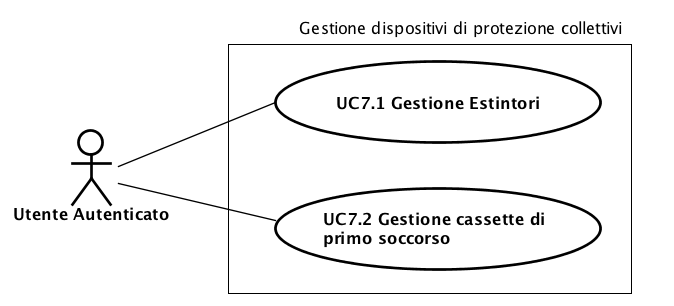
\includegraphics[width=12cm]{Pics/UC7GestioneDispositiviProtezioneCollettivi.png}
				\caption{Diagramma dei casi d'uso relativo alla gestione dei Dispositivi di Protezione Collettiva (DPC).}
				\label{fig:UC7_DPC}
			\end{center}
		\end{figure}
		
		\begin{itemize}
			\item \textbf{Scopo:} Il diagramma presentato nella \autoref{fig:UC7_DPC}, ha lo scopo di rappresentare i casi d'uso necessari al soddisfacimento di tutti i requisiti riguardanti la gestione dei \gls{DPC}\G\ all'interno dell'azienda. \\ 
			\item \textbf{Attori Coinvolti:} Utente Autenticato;
			\item \textbf{Flusso principale degli eventi:} 
			\begin{itemize}
				\item \textit{L'utente autenticato gestisce gli estintori(UC7.1);}
				\begin{itemize}
					\item \textit{L'utente autenticato inserisce un nuovo estintore (UC7.1.1);}
					\item \textit{L'utente autenticato modifica un estintore(UC7.1.2);}
					\item \textit{L'utente autenticato rimuove un estintore (UC7.1.3);}
					\item \textit{L'utente autenticato visualizza tutti gli estintori (UC7.1.4).}
				\end{itemize}
				\item \textit{L'utente autenticato gestisce le cassette di primo soccorso (UC7.2);}
				\begin{itemize}
					\item \textit{L'utente autenticato inserisce una nuova cassetta di primo soccorso (UC7.2.1);}
					\item \textit{L'utente autenticato modifica una cassetta di primo soccorso (UC7.2.2);}
					\item \textit{L'utente autenticato rimuove una cassetta di primo soccorso (UC7.2.3);}
					\item \textit{L'utente autenticato visualizza tutte le cassette di primo soccorso (UC7.2.4).}
				\end{itemize}
			\end{itemize}
		\end{itemize}

\newpage

\subsection{Requisiti}
Al fine di chiarire ciò che si è svolto durante lo stage, è riportata la seguente tabella relativa ai requisiti che devono essere soddisfatti.\\
I requisiti sono stati stesi sulla base di diversi colloqui con il committente e da vincoli interni all'azienda. Dopo ogni  colloquio, è stato steso il relativo verbale.\\ Tutti i requisiti provenienti dai verbali che fanno seguito ai colloqui sono stati catalogati come fonte interna.\\
La codifica di ogni requisito è così composta:
\begin{itemize}
	\item Una \textit{R} iniziale per sottolineare il fatto che si tratta di un requisito;
	\item Un qualificatore del livello di importanza:
	\begin{itemize}
		\item \textit{obb}: obbligatorio;
		\item \textit{des}: desiderabile;
		\item \textit{opz}: opzionale.
	\end{itemize}
	\item Un qualificatore relativo alla tipologia:
	\begin{itemize}
		\item \textit{F}: funzionale;
		\item \textit{Q}: qualitativo;
		\item \textit{V}: vincolo.
	\end{itemize}
	\item Un numero progressivo.
\end{itemize}

\newcolumntype{l}[1]{m{#1}}
\begin{flushleft}
	\begin{tabular}{|l{2cm}|l{8cm}|l{2cm}|}

		\hline
		\textbf{Codice} & \textbf{Descrizione} & \textbf{Fonti} \\
		\hline
		%vincoli
		\label{RobbV0}
		\textit{RobbV0} & Il codice deve essere scritto utilizzando Ruby on Rails. & Azienda \\
		\hline
		%FIGURE DI SISTEMA
		\label{RobbF0}
		\textit{RobbF0} & Un dipendente deve poter ricoprire più cariche contemporaneamente. & fonte interna, \hyperref[section:UC1]{UC1}\\
		\hline
		\label{RdesF1}
		\textit{RobbF1} & Un dipendente deve poter ricoprire una carica in un dato luogo. & fonte interna, \hyperref[section:UC1]{UC1}\\
		\hline
		\label{RobbF1.1}
		\textit{RobbF1.1} & Per ogni carica di ogni dipendente devono essere gestite le informazioni relative alla nomina. & fonte interna, \hyperref[section:UC1]{UC1},\\
		\hline
		\label{RobbF1.2}
		\textit{RobbF1.2} & Per ogni carica di ogni dipendente devono essere segnalate eventuali formazioni mancanti per poterla ricoprire. & fonte interna, \hyperref[section:UC1]{UC1}\\
		\hline
		\label{RobbF1.3}
		\textit{RobbF1.3} & Un \gls{ASPP}\G\ oppure un \gls{RSPP}\G\ deve poter essere sia un membro interno sia esterno all'azienda. & fonte interna, \hyperref[section:UC1]{UC1}, \hyperref[section:UC1_1]{UC1.1} \\
		\hline
		\label{RobbF1.4}
		\textit{RobbF1.4} & Tutte le informazioni relative alle \textit{figure di sitema} devono essere gestibili in un unica sezione. & fonte interna\\
		\hline
		%DPI
		\label{RobbF2}
		\textit{RobbF2} & Un utente amministratore deve poter gestire le tipologie di \gls{DPI}\G\ messe a disposizione dal sistema. & fonte interna, \hyperref[section:UC2_1]{UC2.1}\\
		\hline
		\label{RobbF2.1}
		\textit{RobbF2.1} & Un utente autenticato deve poter aggiungere un \gls{DPI}\G\ alla dotazione di un dipendente  selezionandolo esclusivamente tra quelli messi a disposizione da \hyperref[RobbF2]{RobbF2}. &  \hyperref[section:UC2_1]{UC2.2.1}\\
		\hline
		\label{RobbF2.2}
		\textit{RobbF2.2} & Un utente autenticato deve poter inserire le informazioni aggiuntive relative ad ogni \gls{DPI}\G\ di ogni dipendente. & fonte interna, \hyperref[section:UC2_2]{UC2.2.3}\\
		\hline
		\label{RdesF2.3}
		\textit{RdesF2.3} & La scadenza di un \gls{DPI}\G\ deve essere segnalata con trenta giorni di preavviso. & fonte interna \\
		\hline
		%MANSIONI
		\label{RobbF3}
		\textit{RobbF3} & Un utente amministratore deve poter gestire le denominazioni delle mansioni messe a disposizione dal sistema. & UC3.1\\
		\hline
		\label{RobbF3.1}
		\textit{RobbF3.1} & Un utente autenticato deve poter assegnare una mansione ad un dipendente selezionandola esclusivamente tra le denominazioni messe a disposizione da \hyperref[RobbF3]{RobbF3}. & UC3.2.1 \\
		\hline
		\label{RobbF3.2}
		\textit{RobbF3.2} & Un utente autenticato deve poter inserire le informazioni aggiuntive relative ad ogni mansione assegnata ad ogni dipendente. & UC3.2.3\\
		\hline
	\end{tabular}
\end{flushleft}
\newpage

\begin{flushleft}
	\begin{tabular}{|l{2cm}|l{8cm}|l{2cm}|}
		\hline
		\textbf{Codice} & \textbf{Descrizione} & \textbf{Fonti} \\
		\hline
		%FORMAZIONI
		\label{RobbF4}
		\textit{RobbF4} & Un utente amministratore deve poter gestire le denominazioni delle formazioni messe a disposizione dal sistema. &  fonte interna, \hyperref[section:UC4_1]{UC4.1}\\
		\hline
		\label{RobbF4.1}
		\textit{RobbF4.1} & Un utente autenticato deve poter inserire una formazione di un dipendente selezionandola esclusivamente tra le denominazioni messe a disposizione da \hyperref[RobbF4]{RobbF4}. &  fonte interna, UC4.2.1 \\
		\hline
		\label{RobbF4.2}
		\textit{RobbF4.2} & Un utente autenticato deve poter inserire le informazioni aggiuntive relative ad ogni formazione conseguita da ogni dipendente. & fonte interna, UC3.2.3\\
		\hline
		% soddisfatto
		\label{RdesF4.3}
		\textit{RdesF4.3} & Un utente amministratore deve poter inserire le formazioni necessarie allo svolgimento di una data mansione. & fonte interna \\
		\hline
		%non soddisfatto
		\label{RdesF4.4}
		\textit{RdesF4.4} & La mancanza delle formazioni necessarie per poter svolgere una mansione deve essere segnalata. & fonte interna \\
		\hline
		\label{RobbQ5}
		\textit{RdesQ5} & Deve essere previsto un aiuto all'utente nella compilazione di un  questionario con una quantità rilevante di domande. & Azienda \\
		\hline
		\label{RobbF6}
		\textit{RobbF6} & Devono essere gestite in una apposita sezione le procedure aziendali che compongono il \gls{DVR}\G. & fonte interna, \hyperref[section:UC5]{UC5}\\
		\hline
		\label{RobbF6.1}
		\textit{RobbF6.1} & Devono essere poste tutte le domande che compongono le procedure di prassi fornite dall'\gls{INAIL}\ agli asseveratori. &  fonte interna, \hyperref[section:UC5]{UC5}\\
		\hline
		\label{RdesF7}
		\textit{RobbF7} & Un utente autenticato deve poter gestire le segnalazioni all'organo di vigilanza. & fonte interna,  \hyperref[section:UC6]{UC6}\\
		\hline
		\label{RobbF8}
		\textit{RobbF8} & Deve essere possibile gestire i  \gls{DPC} aziendali indicati in estintori e cassette di primo soccorso. & fonte interna, \hyperref[section:UC7]{UC7}\\
		\hline
		\label{RobbF8.1}
		\textit{RobbF8.1} & Deve essere possibile associare un \gls{DPC} ad una sede o ad un cantiere. & fonte interna\\
		\hline
		\label{RobbF9}
		\textit{RobbF9} & Deve essere possibile impostare regole di validazione delle informazioni inserite condizionata dal valore o la presenza di altre . & fonte interna\\
		\hline
		\label{RdesQ9.1}
		\textit{RopzQ9.1} & Devono essere disponibili degli script che caricano le informazioni minime funzionali all'installazione del sistema. & fonte interna\\
		\hline
		\label{RdesF9.2}
		\textit{RopzF9.2} & Un utente amministratore deve poter impostare regole di validazione da un editor \gls{WYSIWYG} . & Azienda \\
		\hline
		\label{RdesQ10}
		\textit{RdesQ10} & Stesura della documentazione relativa al codice prodotto. & Azienda \\
		\hline
	\end{tabular}
\end{flushleft}
